\documentclass[12pt]{article}
\usepackage{algos-tasks}

\begin{document}
\task[regular]{Square Piling}

\begin{question}
Your friend wants to play a variation of Tetris called Square Piling. You are given a grid $G$ with $n$ rows and $m$ columns for $m \leq n$. The game has $n$ turns. Each turn, you add a $1\times1$ tile to one of the columns. The $i$th turn is defined by $c_i$, the column the tile is stacked in. Each column accumulates tiles; the below grid is an example of a tiled grid for $n = 6$ and $m = 2$. The diagram below implies that $c_i = 1$ for two distinct values of $i$, and that $c_i = 2$ for four distinct values of $i$. 

\begin{center}
    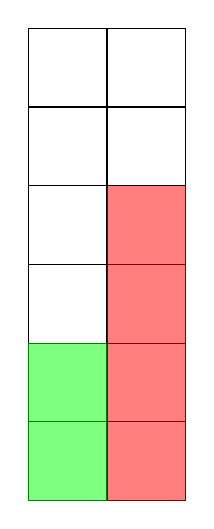
\begin{tikzpicture}
        \draw[step=1.0] (0.0,0.0) grid (2.0,6.0);
        \fill[green, opacity=0.5] (0.0,0.0) rectangle ++(1.0,2.0);
        \fill[red, opacity=0.5] (1.0,0.0) rectangle ++(1.0,4.0);
  \end{tikzpicture}
\end{center}

Your friend is curious about the grid's \emph{completeness} after each turn. A grid's \emph{completeness} is the least number of tiles in one of the grid's columns. For example, the completeness of the tiling of the example grid is 2. An \emph{ideal turn} is a turn $i$ such that the grid's completeness after turn $i$ is strictly greater than the grid's completeness after turn $i-1$. 

Your friend wants you to design an algorithm that counts the number of ideal turns during a Square Piling game because the player who achieves the most ideal turns wins.

\begin{enumerate}
	\item Now, your friend is concerned about the space complexity of the algorithm and has devised the following algorithm that has $O(m)$ space complexity.
 
 \begin{quote}
    We maintain a frequency table $f$ to keep track of the number of tiles in each column from $1$ to $m$ inclusive. This array is zero-initialised. We also maintain a counter $r$ of the number of zero values in the frequency table (initially $m$).
    
    At the $i$th turn, add one to $f[c_i]$ (the number of tiles in $c_i$th column), and if this frequency changes from zero to nonzero, also subtract one from $r$. If $r$ becomes zero as a result: report an ideal turn; subtract one from all frequencies; and recalculate $r$ by iterating over the array $f$.
\end{quote}
 
 However, your friend is unsure whether their algorithm is $O(n)$. Therefore, your new task is to analyse your friend's algorithm:
     
\begin{enumerate}
     \item  Suppose the next turn is the $i$th turn. What is the time complexity of a step which \emph{does not} find an ideal turn? 
     \item Suppose the next turn is the $i$th turn.  What is the time complexity of a step which \emph{does} find an ideal turn?
    \item What is the maximum number of ideal turns there can be in terms of $n$ and $m$?
    
    \item Therefore, what is the time complexity of the entire algorithm?

    This is an example of \emph{amortisation}, where a single operation may be slow but the sequence of operations is guaranteed to be fast.
    
    \textbf{Hint}: The time complexity should account for setting up array $f$, as well as the time spent at each ideal turn \emph{and} at each not ideal turn.
\end{enumerate}
\end{enumerate}
\end{question}

\begin{rubric}
\begin{enumerate}
\item In parts (i) and (ii), account for the operations conducted in such a step, and state the time complexity using big-Oh notation.

In part (iii), calculate the maximum number of ideal turns in terms of $n$ and $m$, with reference to the completeness of the grid $G$.

In part (iv), combine your answers from the previous parts to analyse the time complexity of the entire algorithm. Make sure to also account for any steps earlier in the algorithm that take more than constant time.

    Expected response length: a sentence or short paragraph for each part.
\end{enumerate}
\end{rubric}
\begin{solution}
\end{solution}
\begin{attribution}
    
\end{attribution}
\end{document}